\chapter{E-puck2 Simulation and \acs{ros2} Interface}
\label{chap:simulation}
\shorttitle{\nameref{chap:simulation}}

As previously explained, one of the project's objective is to create \ac{ros2} interface for e-puck2 simulated robot. Even though creating \ac{ros2} interface for Webots robots is automated later in the project, specific \ac{ros2} driver for the e-puck2 in Webots is created first. For us as developers, creating the specific \ac{ros2} driver was necessary to understand better building blocks that can be generalized later. To readers, this chapter will help better understand improvements brought by generalization (see Chapter \ref{chap:generalization}). It will also show that some devices cannot be generalized, e.g., distance sensors cannot feed the \texttt{LaserScan} topic.

\section{Introduction}

Before going to implementation details, it is important to understand the controller's concept in Webots and how it fits in \ac{ros2} driver for Webots simulated robots. The Webots controller controls actuators and reads data from sensors available in a robot. The controller is a "brain" of the robot; it makes the robot move and senses the environment. It consists of two parts, the Webots \ac{api}, which communicates with the simulation and user-defined code that uses the \ac{api} to control the robot. The Webots \ac{api} communicates with the Webots simulation through pipes, a type of inter-process communication \cite{kashyian_portable_2008}. Therefore, there are two processes that run independently, Webots controller and Webots simulation (see Fig. \ref{fig:simulation:webots_user_code_and_api}).

\begin{figure}[H]
    \centering
    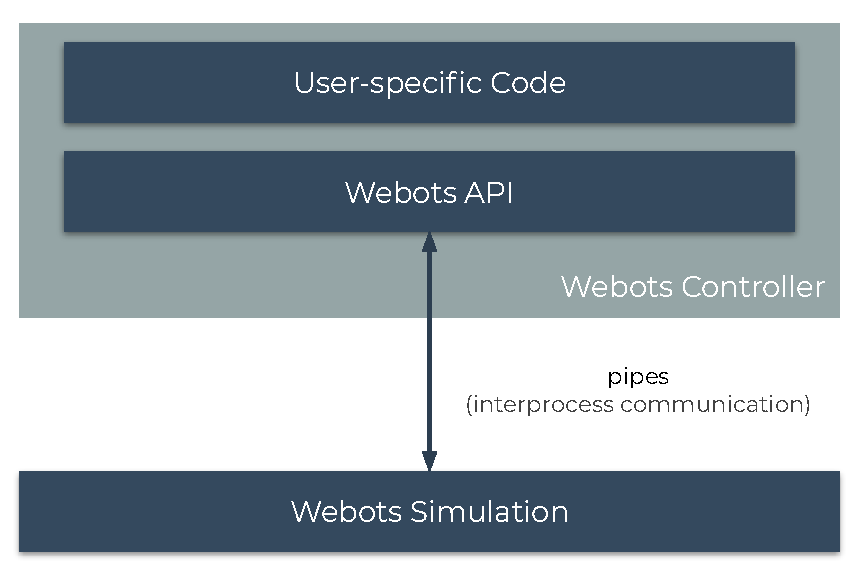
\includegraphics[width=0.8\textwidth]{simulation/figures/webots_user_code_and_api.pdf}
    \caption{User specific code, \ac{api} and simulation within Webots}
    \label{fig:simulation:webots_user_code_and_api}
\end{figure}

In this chapter, a logic that performs translation from Webots \ac{api} to \ac{ros2} \ac{api} will be implemented as a user-specific code (block \textit{User-specific Code} in Fig. \ref{fig:simulation:webots_user_code_and_api}).
Therefore, a block \textit{Webots Controller} from the figure will be referenced as \ac{ros2} driver in the further text.

\section{Webots within \ac{ros2}}
Previously, a term \ac{ros2} driver in scope of Webots is defined. But now, we should define how the \ac{ros2} driver and Webots simulation are executed within \ac{ros2} application. To run the \ac{ros2} driver and Webots to interact with the rest of \ac{ros2} system we can simply put \ac{ros2} libraries to \texttt{PATH}, start the Webots simulation, execute the \ac{ros2} driver and start needed \ac{ros2} nodes.

However, to better integrate Webots into \ac{ros2} launch files\footnote{Launch files in scope of \ac{ros2} are purely documented. Good documentation to understand the core concepts (although not completely accurate) can be found in \ac{ros2} design specification at \url{https://design.ros2.org/articles/roslaunch.html}. A superficial explanation, hiding core concepts, on the usage of the launch files, is given in \ac{ros2} tutorials at \url{https://index.ros.org/doc/ros2/Tutorials/Launch-system/}} are used. The launch files in \ac{ros2} allow user to execute multiple processes (often \ac{ros2} nodes) at once. The launch files are described with Python scripts, and there are three important concepts:
\begin{itemize}
    \item Actions: They represent an intention to do something, like start a process (usually \ac{ros2} nodes), set a parameter, or push a namespace. 
    \item Substitutions: Define a transformable expression that means that the expression contains a placeholder that can be replaced. For example, the substitution can be a path to a file in which filename is again a substitution.
    \item Events: Actions can produce subscribable events. For example, when a process is closed, it will emit an event on which we can close the whole \ac{ros2} application.
\end{itemize}

Using those three concepts minimal launch file containing Webots and \ac{ros2} driver is created (see Fig. \ref{fig:simulation:webots_launch}).

\begin{figure}[H]
    \centering
    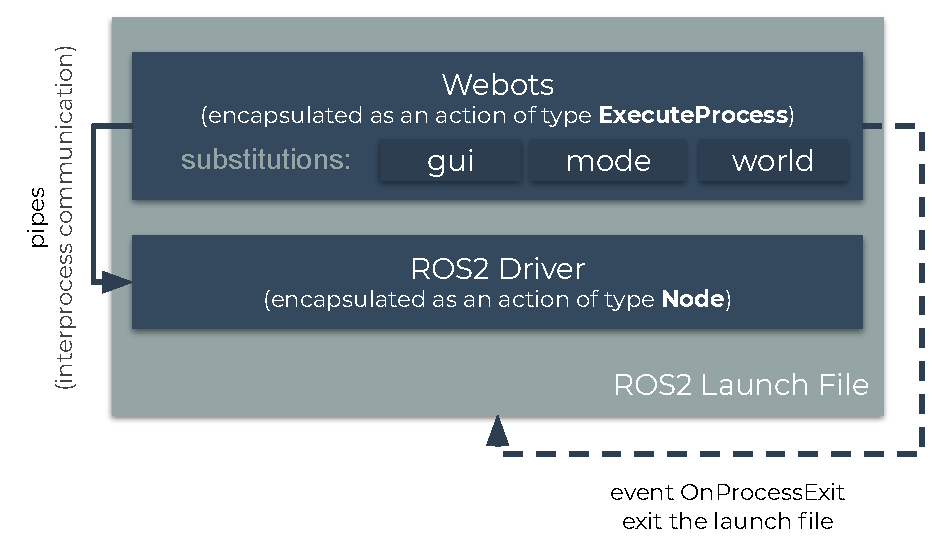
\includegraphics[width=\textwidth]{simulation/figures/webots_launch.pdf}
    \caption{Webots and \ac{ros2} driver within the launch file}
    \label{fig:simulation:webots_launch}
\end{figure}

It will start Webots with three substitutions, \texttt{gui}, \texttt{mode} and \texttt{world} which are used to configure Webots. These substitutions are taken from arguments (as \texttt{LaunchConfiguration}). Also it defines action which will kill the launch file if a user exit the simulation.

The whole implementation is later completely hidden from the user (in Chapter \ref{chap:generalization}).

% TODO: Explain clock synchronization

\section{Covered Sensors and Actuators}

In this section, the implementation of \ac{ros2} driver for the simulated e-puck2 robot is explained. Please note that only the first section (section \label{sec:simulation:odometry_velocity}) will provide the comprehensive explanation. The other sections will briefly cover the implementation details. 

\subsection{Differential Drive}
\label{sec:simulation:odometry_velocity}

Using data from sensors such as wheel encoders, camera, or \ac{imu}, or fusing them, one can estimate the change in position robot's overtime \cite{shen_localization_2011, nister_visual_2004}. With the dead reckoning method, the change in position can be accumulated, and in that way, the robot's position in the local frame (frame relative to robot's start position) can be estimated \cite{ben-ari_elements_2018, astolfi_exponential_1999}. In \ac{ros}, each sensor used for odometry should publish messages of type \texttt{nav\_msgs/Odometry}, and messages from different sensors later can be fused to increase accuracy. 

In the scope of the project, only wheel encoders are used for odometry. Furthermore, e-puck2 does not have encoders but step motors. However, since we can control steps, precisely that data can be used for odometry calculation.

\begin{figure}[H]
    \centering
    \begin{subfigure}[b]{0.9\textwidth}
        \dirtree{%
            .1 nav\_msgs/Odometry.
            .2 (std\_msgs/Header) header.
            .2 (string) child\_frame\_id.
            .2 (geometry\_msgs/PoseWithCovariance) pose.
            .3 (geometry\_msgs/Pose) pose.
            .4 (geometry\_msgs/Point) position.
            .4 (geometry\_msgs/Quaternion) orientation.
            .3 (float64[36]) covariance.
            .2 (geometry\_msgs/TwistWithCovariance) twist.
            .3 (geometry\_msgs/Twist) twist.
            .4 (geometry\_msgs/Vector3) linear.
            .4 (geometry\_msgs/Vector3) angular.
            .3 (float64[36]) covariance.
        }
    \end{subfigure}
    \caption{\texttt{nav\_msgs/Odometry} message type definition in \ac{ros2}}
    \label{fig:simulation:odometry}
\end{figure}

In Fig. \ref{fig:simulation:odometry}, odometry format proposed by \ac{ros2} and used by the community packages is given. It requires \texttt{geometry\_msgs/Pose} (position and orientation) of the robot to be specified, as well as \texttt{geometry\_msgs/Twist} (linear and angular velocity).

First we express velocity of left ($v_left$) and right ($v_right$) wheel by multiplying wheel radius ($R$) with angular velocity:
\begin{equation}
\begin{aligned}
    v_{left} = R \frac{\gamma_{left}(n) - \gamma_{left}(n-1)}{\Delta t} \\
    v_{right} = R \frac{\gamma_{right}(n) - \gamma_{right}(n-1)}{\Delta t}
\end{aligned}
\end{equation}
in which $ \gamma_{left}(n) $ and $ \gamma_{right}(n) $ are angular positions of left and right wheel respectively at the sample $ n $.

For differential drive robots we can simply express linear ($v$) and angular ($\omega$) velocity as:
\begin{equation}
\begin{aligned}
    v = \frac{v_{left} + v_{right}}{2}  \\
    \omega = \frac{v_{right} - v_{left}}{L}
\end{aligned}
\end{equation}
where $ L $ is axle length (distance between the left and the right wheel). The velocity of the robot in odometry frame is given by:
\begin{equation}
\begin{bmatrix}
\dot{x} \\
\dot{y} \\
\dot{\theta}
\end{bmatrix} = \begin{bmatrix}
v \cos(\theta) \\
v \sin(\theta) \\
\omega
\end{bmatrix}
\end{equation}

Knowing the angular and linear velocity, we can integrate it to obtain a position.

\begin{figure}[H]
    \centering
    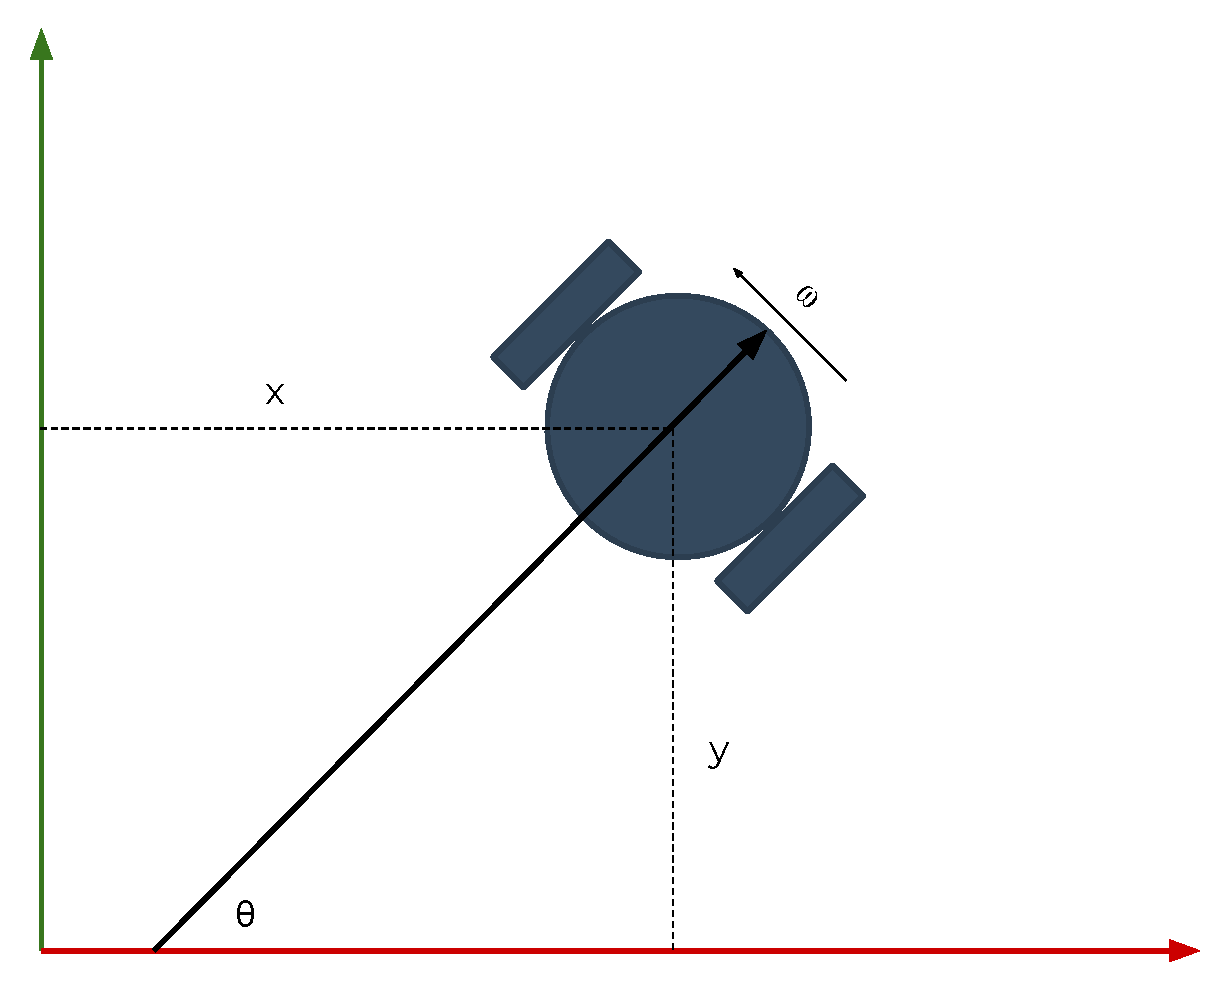
\includegraphics[width=0.8\textwidth]{simulation/figures/odometry.pdf}
    \caption{Robot in local frame \cite{noauthor_16-311_nodate}}
    \label{fig:simulation:odometry_schema}
\end{figure}

As it is a non-linear system of differential equations we can integrate it using one of the methods for the numeric integration. It can simply be integrated using Euler method expressed in general terms as:
\begin{equation}
    y(t + h) \approx y(t) + h y'(t)
\end{equation}
This method would be computationally cheap, but not as accurate as for example fourth order of Runge-Kutta \cite[p. 40]{noauthor_solving_1993}. The choice of the method for the numerical integration is mainly based on sample rate we perform with Pi-puck extension. In case of e-puck2 physical robot, communication with the on-board \ac{mcu} is configured exchange data with pi-puck extension at around 20Hz. Considering the slow sample rate and the computational power of the Raspberry Pi Zero to handle floating-point operations it is reasonable to choose the fourth order of Runge-Kutta over Euler method and trade computation resources for better accuracy. Therefore, we express the numerical integration as following:


\begin{equation}
\begin{aligned}
    & k_{00} = v \cos{\theta_{n-1}} \\
    & k_{01} = v \sin{\theta_{n-1}} \\
    & k_{02} = \omega \\
    & \\
    & k_{10} = v \cos{\theta_{n-1} + \frac{t}{2}k_{02}} \\
    & k_{11} = v \sin{\theta_{n-1} + \frac{t}{2}k_{02}} \\
    & k_{12} = \omega \\
    & \\
    & k_{20} = v \cos{\theta_{n-1} + \frac{t}{2}k_{12}} \\
    & k_{21} = v \sin{\theta_{n-1} + \frac{t}{2}k_{12}} \\
    & k_{22} = \omega \\
    & \\
    & k_{30} = v \cos{\theta_{n-1} + t k_{22}} \\
    & k_{31} = v \sin{\theta_{n-1} + t k_{22}} \\
    & k_{32} = \omega
\end{aligned}
\end{equation}

\begin{equation}
\begin{aligned}
    \begin{bmatrix}
        x_n \\
        y_n \\
        \theta_n
    \end{bmatrix} = \begin{bmatrix}
        x_{n-1} \\
        y_{n-1} \\
        \theta_{n-1}
    \end{bmatrix} + \frac{t}{6}
    \begin{bmatrix}
        k_{00} + 2 (k_{10} + k_{20}) + k_{30} \\
        k_{01} + 2 (k_{11} + k_{21}) + k_{31} \\
        k_{02} + 2 (k_{12} + k_{22}) + k_{32}
    \end{bmatrix} 
\end{aligned}
\end{equation}

Notice in Fig. \ref{fig:simulation:odometry} that the orientation is represented as a quaternion while our orientation is represented Euler angles. To convert the Euler angles to quaternions we reference to \cite[p. 12]{diebel_representing_2006}: 

\begin{equation}
    \bm{q}(\alpha_x, \alpha_y, \theta) = \begin{bmatrix}
        \cos{\frac{\alpha_x}{2}} \cos{\frac{\alpha_y}{2}} \cos{\frac{\theta}{2}} + \sin{\frac{\alpha_x}{2}} \sin{\frac{\alpha_y}{2}} \sin{\frac{\theta}{2}} \\
        -\cos{\frac{\alpha_x}{2}} \sin{\frac{\alpha_y}{2}} \sin{\frac{\theta}{2}} + \cos{\frac{\alpha_y}{2}} \cos{\frac{\alpha_y}{2}} \sin{\frac{\theta}{2}} \\
        \cos{\frac{\alpha_x}{2}} \cos{\frac{\theta}{2}} \cos{\frac{\alpha_y}{2}} + \sin{\frac{\alpha_x}{2}} \cos{\frac{\alpha_y}{2}} \sin{\frac{\theta}{2}} \\
        \cos{\frac{\alpha_x}{2}} \cos{\frac{\alpha_y}{2}} \sin{\frac{\theta}{2}} - \sin{\frac{\alpha_x}{2}} \sin{\frac{\theta}{2}} \sin{\frac{\alpha_y}{2}}
    \end{bmatrix}
\end{equation}
in which we can neglect $ \alpha_x $ and $ \alpha_y $ as those two elements are always 0 for differential driver robots.

At this point, the obtained $ x, y, \bm{q}, \dot{x}, \dot{y} $ and $ \dot{\theta} $ are packed in \texttt{nav\_msgs/Odometry} (see Fig. \ref{fig:simulation:odometry}) and published periodically at 20Hz.

With \texttt{nav\_msgs/Odometry} messages the rest of the \ac{ros2} is aware of robot's odometry data. However, in addition to odometry data, the odometry frame has to be defined as well to explain the robot's position with respect to the odometry frame. For that purpose \ac{ros2} defines transform messages of type \texttt{geometry\_msgs/TransformStamped} (see Fig. \ref{fig:simulation:transform}). In short, transform messages are used to create a transform tree to keep track of multiple coordinate frames over time. Keeping track of the coordinate frames is an essential aspect of \ac{ros} in general, and it will be properly explained in Chapter \ref{chap:generalization} in which it will be extensively utilized.

\begin{figure}[H]
    \centering
    \begin{subfigure}[b]{0.9\textwidth}
        \dirtree{%
            .1 geometry\_msgs/TransformStamped.
            .2 (std\_msgs/Header) header.
            .2 (string) child\_frame\_id.
            .2 (geometry\_msgs/Transform) transform.
            .3 (geometry\_msgs/Vector3) translation.
            .3 (geometry\_msgs/Quaternion) rotation.
        }
    \end{subfigure}
    \caption{\texttt{geometry\_msgs/TransformStamped} message type definition in \ac{ros2}}
    \label{fig:simulation:transform}
\end{figure}

but to control the robot's velocity a message of type \texttt{geometry\_msgs/Twist} (see Fig. \ref{fig:simulation:twist}) has to be utilized. Therefore, the node has to subscribe to the topic and set the wheels' angular speed accordingly.

\begin{figure}[H]
    \centering
    \begin{subfigure}[b]{0.9\textwidth}
        \dirtree{%
            .1 geometry\_msgs/Twist.
            .2 (std\_msgs/Header) header.
            .2 (geometry\_msgs/Vector3) linear.
            .2 (geometry\_msgs/Vector3) angular.
        }
    \end{subfigure}
    \caption{\texttt{geometry\_msgs/Twist} message type definition in \ac{ros2}}
    \label{fig:simulation:twist}
\end{figure}

The target velocity of the left ($v_{left}$) and right ($v_{right}$) can be obtained as:
\begin{equation}
\begin{aligned}
    & v_{left} = v_{ref} + L \frac{\omega_{ref}}{2} \\
    & v_{right} = v_{ref} - L \frac{\omega_{ref}}{2}
\end{aligned}
\end{equation}
where $ v_{ref}  $ is reference linear velocity (available in the \ac{ros2} message \texttt{.linear.x}) and $ \omega_{ref} $ angular reference velocity (available in the \ac{ros2} message \texttt{.angular.z}). Webots expect the velocity to be given in radians per second (rad/s):
\begin{equation}
\begin{aligned}
    & \omega_{left} = \frac{v_{left}}{R} \\
    & \omega_{right} = \frac{v_{ref}}{R} 
\end{aligned}
\end{equation}

Within this section, a minimal implementation of velocity control and odometry is given. It allows e-puck2 to use the standard \ac{ros2} interface to receive velocity control commands and to publish it's position and other relevant information within the odometry frame. Messages of type \texttt{geometry\_msgs/TransformStamped} are published to topic name \texttt{/tf}, messages of type \texttt{nav\_msgs/Odometry} are published to a topic name \texttt{/odom} and messages of type \texttt{geometry\_msgs/Twist} are received from topic name \texttt{/cmd\_vel}. Those topic names follow \ac{ros2} conventions for topic naming and can be changed using \ac{ros2} remapping\footnote{Tutorial on \ac{ros2} remapping can be found at \url{https://index.ros.org/doc/ros2/Tutorials/Node-arguments/\#id1}}. 

\subsection{Distance Sensors}
E-puck2 is equipped with 8 infra-red sensors and one \ac{tof} sensor (see Fig. \ref{fig:simulation:distance_sensors}). These sensors are modeled as \texttt{DistanceSensor}\footnote{More information about \texttt{DistanceSensor} nodes is available \url{https://cyberbotics.com/doc/reference/distancesensor}} in Webots.

\begin{figure}[H]
    \centering
    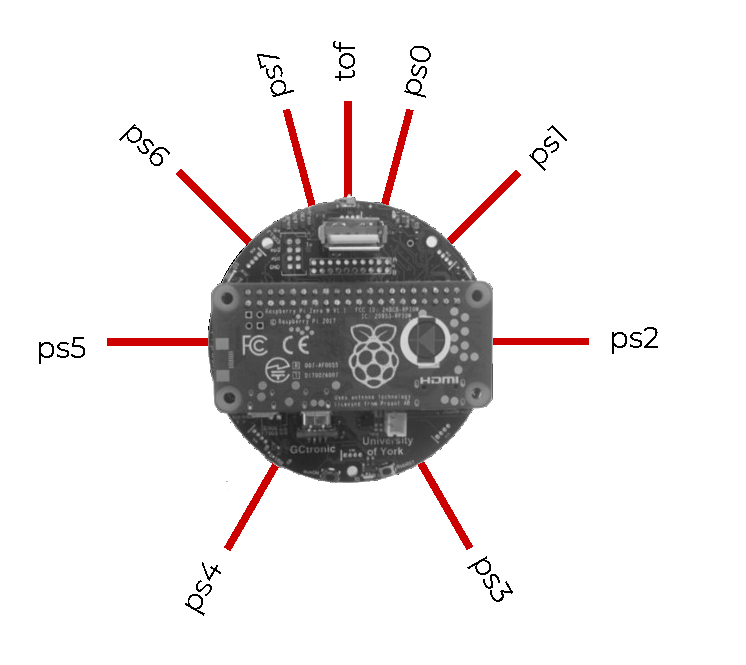
\includegraphics[width=0.65\textwidth]{simulation/figures/distance_sensors.pdf}
    \caption{Distance sensors available on e-puck2}
    \label{fig:simulation:distance_sensors}
\end{figure}

All details about the sensors are obtained from the Webots and published to a topic of type \texttt{sensor\_msgs/Range}\footnote{Definition of \texttt{sensor\_msgs/Range} message type is available at \url{https://github.com/ros2/common_interfaces/blob/master/sensor_msgs/msg/Range.msg}}.

\subsubsection{Laser Scanner}
\ac{ros2} defines \texttt{sensor\_msgs/LaserScan}\footnote{Definition of \texttt{sensor\_msgs/LaserScan} message type is available at \url{https://github.com/ros2/common_interfaces/blob/master/sensor_msgs/msg/LaserScan.msg}} for \acp{lidar} and other types of planar laser range-finders. Those messages are commonly used by \ac{ros2} community packages like \texttt{navigation2} and \texttt{slam\_toolbox}. The message type requires an array of measurements at angles that are equally distanced from each other. 

Therefore, even though there is no \ac{lidar} available on the e-puck2 it is possible to emulate it using available distance sensors. Since the distance sensors are not equally positioned, virtual distance sensors are added to fill space between the actual distance sensors (see Fig. \ref{fig:simulation:laserscan}).

% TODO: Explain https://answers.ros.org/upfiles/14177210732958238.jpg

\begin{figure}[H]
    \centering
    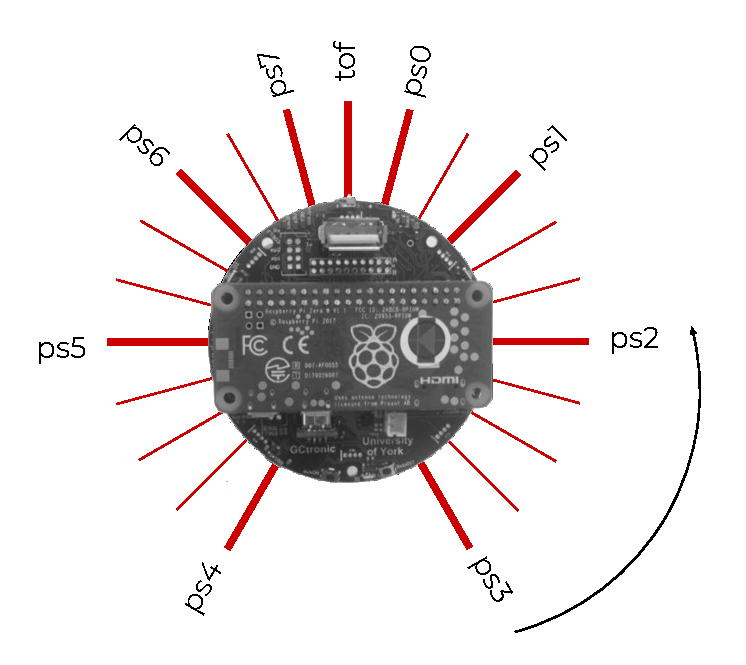
\includegraphics[width=0.8\textwidth]{simulation/figures/laserscan.pdf}
    \caption{Virtual distance sensors are added to emulate \ac{lidar}, making the angle difference between the rays constant ($15^\circ$)}
    \label{fig:simulation:laserscan}
\end{figure}

\subsection{Light Sensors}
E-puck2 has eight infra-red sensors which besides proximity can measure light intensity as well. \ac{ros2} interface for light sensors uses messages of type \texttt{sensor\_msgs/Illuminance}\footnote{Definition of \texttt{sensor\_msgs/Illuminance} message type is available at \url{https://github.com/ros2/common_interfaces/blob/master/sensor_msgs/msg/Illuminance.msg}}. The message type requires the measurements to be in Lux units (illuminance) while measurements acquired in Webots\footnote{Light sensors in Webots are represented as \texttt{LightSensor} node - \url{https://cyberbotics.com/doc/reference/lightsensor}} are expressed in watts per square meter [$W/m^2$] (irradiance). The conversion is done according to \cite{michael_conversion_2019}.

\subsection{\acl{imu}}
\ac{imu} in Webots modeled as two nodes, \texttt{Accelerometer} and \texttt{Gyro}. Measurements from those two nodes are combined and packed into messages of type \texttt{sensor\_msgs/Imu}.

\subsection{Camera}
Typically, cameras in \ac{ros2} use two topics, one for data (images) and another one for intrinsic camera parameters. Images from Webots camera node are sampled, packed in \ac{ros2} messages of type \texttt{sensor\_msgs/Image} and published repeatedly. The intrinsic parameters are defined by \ac{ros2} has the following form:
\begin{equation}
K = \begin{bmatrix}
    f_x & 0 & c_x \\
    0 & f_y & c_y \\
    0 & 0 & 1
\end{bmatrix}
\end{equation}

Webots doesn't provide such matrix, but it is easy to create one from the existing parameters. Since Webots camera doesn't provide distortions that move the focal length then $f_x = f_y$ and it is equal to the focal length that can be obtained in Webots (e.g. \texttt{getFocalLength()}). The principal point also doesn't have offset, but it is in the center of the image $c_x$ is equal to $ \frac{\texttt{image\_width}}{2} $ and $c_y$ is equal to $ \frac{\texttt{image\_height}}{2} $.

\subsection{\acsp{led}}
There are eight \acsp{led} available in the robot and they are controlled with messages of type \texttt{std\_msgs/Int32}. The last three bytes of the value are used to set three \ac{rgb} components in case of \acsp{rgbled} and for the regular \acp{led} the value is used to set the intensity.

\subsection{Final Interface}

In the table bellow (see Table \ref{tab:simulation:complete_interface}) the final interface is shown.

\begin{table}[H]
    \begin{adjustwidth}{-1.5in}{-1.5in}
    \centering
    \begin{tabular}{|l|l|l|}
        \hline
        \textbf{Topic name} & \textbf{Message type} & \textbf{Description} \\
        \hline
        \texttt{/cmd\_vel} & \texttt{geometry\_msgs/Twist} & Controls robot's velocity \\
        \hline
        \texttt{/odom} & \texttt{nav\_msgs/Odometry} & Odometry measurements from wheels \\
        \hline
        \texttt{/ps[0-7]} & \texttt{sensor\_msgs/Range} & Measurements from infra-red sensors \\
        \hline
        \texttt{/tof} & \texttt{sensor\_msgs/Range} & Measurements from \acs{tof} sensor \\
        \hline
        \texttt{/scan} & \texttt{sensor\_msgs/LaserScan} & Emulated \ac{lidar} measurements \\
        \hline
        \texttt{/ls[0-7]} & \texttt{sensor\_msgs/Illuminance} & Light measurements from infra-red sensors \\
        \hline
        \texttt{/imu} & \texttt{sensor\_msgs/Imu} & Measurements from \acs{imu} \\
        \hline
        \texttt{/led[0-7]} & \texttt{std\_msgs/Int32} & Controls \acsp{led} \\
        \hline
        \texttt{/gs[0-2]} & \texttt{sensor\_msgs/Range} & Measurements from ground sensors \\
        \hline
        \texttt{/image\_raw} & \texttt{sensor\_msgs/Image} & Camera images \\
        \hline
        \texttt{/camera\_info} & \texttt{sensor\_msgs/CameraInfo} & Camera intrinsic parameters \\
        \hline
        \texttt{/tf} & \texttt{tf2\_msgs/TFMessage} & Dynamic transforms \\
        \hline
        \texttt{/tf\_static} & \texttt{tf2\_msgs/TFMessage} & Static transforms \\
        \hline
    \end{tabular}
    \caption{Complete \ac{ros2} interface for e-puck2 robot}
    \label{tab:simulation:complete_interface}
    \end{adjustwidth}
\end{table}

In addition to the previously mentioned topics, there are topics with name \texttt{/gs[0-2]}, and those topics publish data from ground sensors. The ground sensors can be bought as a separate e-puck2 module. Therefore, this part of the \ac{ros2} interface will be automatically created if the module is present in the e-puck.

Another topic not mentioned before is \texttt{/tf\_static}. It is used to describe transformations between different coordinate frames that do not typically change (for example, a transformation between the robot's base and the \ac{lidar}). Messages published to this topic have specific \ac{qos} configured, durability is set to be transient local. The transient local \ac{qos} means that the nodes joined to the system will receive the messages even though the messages are published much earlier. Avoiding periodic publishing reduces the load on the \ac{ros2} driver as the messages have to be published only once.

Another performance improvement is made by not publishing the messages all the time. The messages are published only if the subscribers are available. It significantly improves performance, especially in the camera's case, as it is very \acs{cpu}/\acs{gpu} intensive task.

% TODO: Continious Integration